\documentclass{article}
\usepackage[T1]{fontenc}
\usepackage{helvet}
\renewcommand\familydefault{\sfdefault}
\usepackage[a4paper, left=2.5cm, right= 2.5cm, top=2.5cm, bottom= 2.5cm]{geometry} %cambiar los márgenes
\usepackage{amsmath, amssymb, cancel, extarrows, amsthm }%símbolos matemáticos
\usepackage{wasysym}  %la carita triste
\usepackage{derivative}
\usepackage{physics}
\usepackage{polynom}
\usepackage{graphicx, wrapfig}% Include figure files
\usepackage{subfig}
\usepackage{dcolumn}% Align table columns on decimal point
\usepackage{bm}% bold math
\usepackage{hyperref}% add hypertext capabilities
\usepackage{units}
\usepackage{fancyhdr, ragged2e}
\setlength{\headheight}{13.07002pt}
\renewcommand{\footrulewidth}{0.4pt}
\usepackage{float}
\usepackage{booktabs}
\usepackage{multirow}
\usepackage{multicol}
\usepackage[table,xcdraw]{xcolor}
\usepackage{xcolor, colortbl}
\usepackage{pagecolor}
\usepackage{tcolorbox}
\newtcolorbox{mybox}{colback=gray!5!white,colframe=black!75!black}
\definecolor{cadetblue4}{rgb}{.33,.53,.55}
\definecolor{azulcrepuscular}{rgb}{.49,.62,.75}
\definecolor {atomictangerine} {rgb} {1.0, 0.6, 0.4}
\usepackage{longtable}
\usepackage{hyperref}
\hypersetup{
    colorlinks=true,
    linkcolor=black,
    filecolor=magenta,      
    urlcolor=blue,
    pdftitle={Overleaf Example},
    pdfpagemode=FullScreen,
    }


\title{\textbf{EvAU 2023:} Matemáticas II}
\date{7 de junio, 2023\\
\noindent\rule{\textwidth}{0.5pt}}
\author{Manuel Lozano Bermúdez}
    
\begin{document}
\maketitle

\section*{Opción A:}
\begin{mybox}
    \paragraph{A.1-}En una obra, para transportar la tierra extraída para la construcción de los cimientos de un edificio, se usan tres
    tipos de camiones diferentes: $A$, $B$ y $C$. Los camiones de tipo $A$ tienen una capacidad de 14 toneladas, los de
    tipo $B$, de 24 toneladas y los de tipo $C$, de 28 toneladas. Habría que traer un camión más de tipo $A$ para igualar
    al número de camiones restantes. El $10\%$ de la capacidad de todos los camiones tipo $B$ supone un séptimo de la
    de los de mayor tonelaje. Hoy, realizando un único viaje cada camión a máxima capacidad, se han extraído de la
    obra 302 toneladas de tierra. ¿Cuánta tierra ha sido transportada hoy por los camiones de cada tipo? 
\end{mybox}

\paragraph{Solución:} 
En primer lugar, llamaremos al número de camiones de cada tipo $A,B,C$, respectivamente; y la capacidad total de esos camiones será la capacidad de un camión individual por el número de camiones de cada tipo. En forma de tabla, esto es:
\begin{table}[!h]
    \centering
    \begin{tabular}{c|c|c|c}
         $\#$ Camiones& $A$&$B$&$C$  \\ \hline
         Capacidades& $14A$&$24B$&$28C$ 
    \end{tabular}
    \label{tab:my_label}
\end{table}\\
Como la capacidad total de todos los camiones (la suma de la segunda fila) tiene que ser 302 toneladas, obtenemos una primera ecuación.
\begin{equation}
    \boxed{14A+24B+28C=302}
\end{equation}
Por otro lado, para que el número de camiones de tipo $A$ sea igual al número de camiones de los tipos restantes, necesitamos añadir un camión de tipo $A$ a los que ya tenemos. Esto es nuestra segunda ecuación.
\begin{equation}
    \boxed{A+1=B+C}
\end{equation}
Por último, sabemos que el $10\%$ de la capacidad de $B$ ($10\%$ de $24B$) supone un séptimo de la capacidad de los camiones de \emph{mayor} tonelaje, es decir, la capacidad de $C$ ($28C$). Con esto obtenemos nuestra última ecuación.
\begin{equation}
    10\% \text{ de } 24B=\frac{1}{7} \text{ de } 28C\implies \boxed{2.4B=4C}
\end{equation}
Y tenemos finalmente un sistema de ecuaciones lineales con tres incógnitas:
$$
\left \{ \begin{array}{ccccc}
     14A&+\phantom{.}24B  &+28C&=&302  \\
     \phantom{14}A  &-\phantom{24}B    &-\phantom{28}C  &=&-1\\
        & \phantom{-}2.4B &-\phantom{8}4C &=&0
\end{array} \right .
$$
Este sistema puede resolverse de muchas maneras. En este caso, empleo la eliminación gaussiana. En forma matricial:
$$
\left [ \begin{array}{ccc|c}
    14 &24&28&302  \\
    1 & -1&-1&-1   \\
    0& 2.4& -4 &0
\end{array} \right ] \xlongrightarrow{F_2'=14 F_2 -F_1} \left [ \begin{array}{ccc|c}
    14 &24&28&302  \\
    0 & -38&-42&-316   \\
    0& 2.4& -4 &0
\end{array} \right ]\xlongrightarrow{F_3'=(38/2.4) \ F_3 +F_2}
$$
\begin{align*}
\left [ \begin{array}{ccc|c}
    14 &24&28&302  \\
    0 & -38&-42&-316   \\
    0& 0& -316/3 &-316
\end{array} \right ] \longrightarrow \left \{ \begin{array}{c}
     -(316/3) \ C=-316  \\
     \implies C=3
\end{array} \right . &\longrightarrow \left \{ \begin{array}{c}
     -38B-42C=-316  \\
     \implies B=5
\end{array} \right .\\ &\longrightarrow \left \{ \begin{array}{c}
     14A+24B+28C=302  \\
     \implies A=7 
\end{array} \right .
\end{align*}
Como nos preguntan cuánta tierra ha sido transportada por cada tipo de camión, el resultado final será: $A: 14\times 7=98$ t, $B: 24\times 5=120$ t y $C: 28\times 3=84$ t.\\

\noindent\rule{\textwidth}{0.5pt}
\begin{mybox}
    \paragraph{A.2-} Dada la función $f(x)=\sqrt[3]{(x^2-1)^2}$, se pide:
    \begin{enumerate}
        \item[(a)] Estudiar si es par o impar.
        \item[(b)] Estudiar su derivabilidad en el punto $x=1$.
        \item[(c)] Estudiar sus extremos relativos y absolutos.
    \end{enumerate}
\end{mybox}
\paragraph{Solución:} $f(x)=\sqrt[3]{(x^2-1)^2}=(x^2-1)^{2/3} \ \ge0$:
\begin{enumerate}
    \item[(a)] Si una función es \emph{par}: $f(-x)=f(x)$. Si una función es \emph{impar}: $f(-x)=-f(x)$.\\
    
    $ f(-x)=\sqrt[3]{((-x)^2-1)^2}=\sqrt[3]{(x^2-1)^2}=f(x)\implies $ La función es \textbf{par.}
    \item[(b)] Para que una función sea derivable en un punto, debe cumplir primero que sea continua en ese punto. Como la función $f(x)$ no tiene problemas de dominio ($D(f)=\mathbb{R}$), es continua en toda la recta real, y por tanto en $x=1$. La condición de derivabilidad es que el límite en $x=1$ de la derivada exista, es decir, $f'(1^+)=f'(1^-)$
    \begin{equation*}
        \begin{split}
            f'(x)&=\frac{2}{3}(x^2-1)^{-1/3}\cdot 2x=\frac{4}{3}\frac{x}{\sqrt[3]{x^2-1}}\\
            &\rightarrow f'(1^+)=\lim_{x\to 1^+} \frac{4}{3}\frac{x}{\sqrt[3]{x^2-1}}=\frac{4}{3}\cdot \frac{1}{0^+}=+\infty\\
            &\rightarrow f'(1^-)=\lim_{x\to 1^-} \frac{4}{3}\frac{x}{\sqrt[3]{x^2-1}}=\frac{4}{3}\cdot \frac{1}{0^-}=-\infty\\
            &\implies \nexists f'(1^\pm) \implies \text{ La función \textbf{no es derivable} en }x=1.
        \end{split}
    \end{equation*}

    \item[(c)] Los extremos \emph{relativos} se estudian igualando la derivada de $f(x)$ a cero y estudiando el crecimiento y decrecimiento de la función.
    \begin{gather*}
        f'(x)=\frac{4}{3}\frac{x}{\sqrt[3]{x^2-1}}\equiv 0\implies \boxed{x=0} \text{ \small  (posible extremo relativo)}.
    \end{gather*}
    Otros puntos a considerar en el crecimiento y decrecimiento de la función son los puntos conflictivos de la derivada, que son $x=\pm 1$ ya que la función no es derivable en esos puntos pero $f(x)$ es continua.
    \begin{table}[!h]
        \centering
        \begin{tabular}{c|c|c|c|c}
           Intervalos  &$(-\infty ,-1)$ & $(-1,0)$     & $(0,1)$     & $(1,+\infty )$  \\ \hline
           $f'(x)$     & $<0$           & $>0$        & $<0$        & $>0$  \\ \hline 
           $f(x)$      &$\searrow $     & $\nearrow $ & $\searrow $ & $\nearrow $ \\
        \end{tabular}
        \label{tab:my_label2}
    \end{table}\\
    En $x=0$, la función alcanza un \textbf{máximo relativo}, cuyo valor es $f(0)=1$. Como la función crece hasta hacerse infinita en $x\to \pm \infty $, \textbf{no hay máximos absolutos}. Con respecto a los mínimos, como la función $f(x) \ge 0 \ \forall x \in \mathbb{R}$, en $x=\pm 1$ la función tiene \textbf{mínimos absolutos} ($f(\pm 1)=0$), y \textbf{no hay mínimos relativos}. 
    \newpage
    Estos resultados que hemos obtenido pueden verse bien en la siguiente gráfica.
    \begin{figure}[!h]
        \centering
        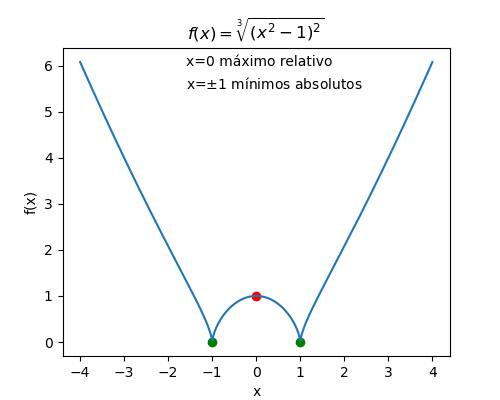
\includegraphics[scale=.7]{evau_2023.png}
        \caption*{$f(x)$ en $[-4,4]$.}
        \label{fig:enter-label}
    \end{figure}
    Como se puede comprobar, la función presenta simetría par. En $x=\pm 1$ la función no es derivable ya que tenemos \emph{picos} (derivadas $\to \pm \infty$) en esos puntos; y presenta un máximo relativo en $x=0$ y mínimos absolutos en $x=\pm 1$.
\end{enumerate}
    
\noindent\rule{\textwidth}{0.5pt}
\begin{mybox}
    \paragraph{A.3-} Sean los puntos $A(1,-2,3)$, $B(0,2,-1)$ y $C(2,1,0)$. Se pide:
    \begin{enumerate}
        \item[(a)] Comprobar que forman un triángulo $T$ y hallar una ecuación del plano que los contiene.
        \item[(b)] Calcular el corte de la recta que pasa por los puntos $A$ y $B$ con el plano $z = 1$.
        \item[(c)] Determinar el perímetro del triángulo $T$. 
    \end{enumerate}
\end{mybox}
\paragraph{Solución:}
\begin{enumerate}
    \item[(a)] Un triángulo está formado por tres lados y tres vértices \emph{que no son colineales}, es decir, que los puntos no están alineados. La manera de comprobar que los puntos $A,B$ y $C$ forman un triángulo es, entonces, comprobar que los puntos no son colineales. Si tres puntos $A,B,C$ \emph{son} colineales, entonces los vectores que forman, $\vec{AB}, \Vec{BC}, \Vec{AC}$ deben ser \emph{linealmente dependientes}. Esto es:
    $$
    \Vec{AB}=\lambda \Vec{AC} 
    $$
    Los vectores $\Vec{AB}$, $\Vec{AC}$ y $\Vec{BC}$ se calculan de la siguiente manera: $\Vec{AB} = B-A=(0,2,-1)-(1,-2,3) = (-1,4,-4)$, $\Vec{AC} = C-A = (2,1,0)-(1,-2,3) = (1,3,-3)$, $\Vec{BC}=C-B=(2,1,0)-(0,2,-1) = (2,-1,1)$. Entonces:
    $$
    \Vec{AB}=(-1,4,-4)=\lambda \Vec{AC}=\lambda (1,3,-3) \implies \begin{cases}
         -1=\lambda \cdot 1    \implies \lambda =-1\\
          4=\lambda \cdot 3    \implies \lambda =4/3\\ 
         -4=\lambda \cdot (-3) \implies \lambda =4/3
    \end{cases}
    $$
    Como no hay un valor de $\lambda$ único, los vectores son linealmente independientes, por lo que los puntos $A,B,C$ \textbf{forman un triángulo}. \\

    Por otro lado, la ecuación del plano que pasa por los tres puntos o, lo que es lo mismo, pasa por el punto $A(a_1,a_2,a_3)$ y tiene como vectores $\Vec{AB}$ y $\Vec{AC}$ es:
    $$
    \pi \equiv \left | \begin{array}{ccc}
        AB_1 & AC_1 & x-a_1  \\
        AB_2 & AC_2 & y-a_2  \\
        AB_3 & AC_2 & z-a_3
    \end{array} \right | =0= \left | \begin{array}{ccc}
        -1 &  1 & x-1  \\
         4 &  3 & y+2  \\
        -4 & -3 & z-3
    \end{array} \right |
    $$
    Calculando el determinante y simplificando, obtenemos que la ecuación del plano $\boxed{\pi \equiv z+y=1}$

    \item[(b)] La recta que pasa por $A$ y $B$ es la recta que pasa por $A$ y tiene un vector $\Vec{AB}=(-1,4,-4)$, que en ecuaciones parametricas es:
    $$
    r\equiv \begin{cases}
        x=1-\lambda \\
        y=-2+4\lambda \\
        z=3-4\lambda 
    \end{cases} \ , \ \lambda \in \mathbb{R}
    $$
    El corte de la recta con este plano es la intersección $r \cap (z=1)\equiv P$.
    $$
    r\cap (z=1) : z=1=3-4\lambda \iff \boxed{\lambda =1/2} \rightarrow \begin{cases}
        x=1-1/2=1/2\\
        y=-2+2=0\\
        z=1
    \end{cases}\implies \boxed{P(1/2,0,1)}
    $$

    \item[(c)] El perímetro del triángulo $T$ se calcula como la suma de los tres lados, es decir:
    \begin{equation*}
        \begin{split}
            p=|\Vec{AB}|+|\Vec{AC}|+|\Vec{BC}|&=\sqrt{1^1+4^2+4^2}+\sqrt{1+3^2+3^2}+\sqrt{2^2+1^2+1^2}\\
                                              &=\sqrt{33}+\sqrt{19}+\sqrt{6} =\boxed{12.55 \text{ u}} 
        \end{split}
    \end{equation*}
\end{enumerate}

\noindent\rule{\textwidth}{0.5pt}
\begin{mybox}
    \paragraph{A.4-} Se tiene un suceso $A$ de probabilidad $P(A) = 0.3$:
    \begin{enumerate}
        \item[(a)] Un suceso $B$ de probabilidad $P(B) = 0.5$ es independiente de $A$. Calcule $P(A \cup B)$. 
        \item[(b)] Otro suceso $C$ cumple $P(C | A) = 0.5$. Determine $P(A \cap \bar{C})$. 
        \item[(c)] Si se tiene un suceso $D$ tal que $P(\Bar{A} | D) = 0.2$ y $P(D | A) = 0.5$, calcule $P(D)$. 
    \end{enumerate}
\end{mybox}
\paragraph{Solución:}
\begin{enumerate}
    \item[(a)] Al ser el suceso $B$ independiente de $A$, entonces $P(A\cap B)=P(A)\cdot P(B)=0.3 \cdot 0.5=0.15$. \\ La probabilidad $P(A\cup B)=P(A)+P(B)-P(A\cap B)=0.3+0.5-0.15=\boxed{0.65}$ 
    \item[(b)] La probabilidad que buscamos está representada en rojo en la siguiente imagen:
    
    \begin{minipage}{.64\textwidth}
    \begin{equation*}
        \begin{split}
            P(A\cap \Bar{C})&=P(A)-P(A\cap C) \\
            P(C|A)&=0.5=\frac{P(A\cap C)}{P(A)}\implies P(A\cap C)=0.15\\
            P(A\cap \Bar{C})&=0.3-0.15=\boxed{0.15}
        \end{split}
    \end{equation*}
    \end{minipage}
    \begin{minipage}{.64\textwidth}
        \setlength{\parindent}{1em}
        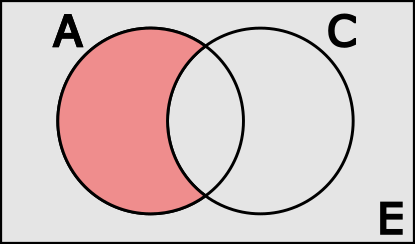
\includegraphics[scale=.4]{g6449.png}
    \end{minipage}

    \item[(c)] $P(\Bar{A}|D)=0.2=\dfrac{P(\Bar{A}\cap D)}{P(D)}=\dfrac{P(D)-P(D\cap A)}{P(D)}$ \small (mismo razonamiento que ap. b) \normalsize\\
    Además:\\
    $
    P(D|A)=0.5=\dfrac{P(D\cap A)}{P(A)}=\dfrac{P(D\cap A)}{0.3}\implies P(D\cap A)=0.15.
    $ Por tanto, obtenemos que:
    \begin{gather*}
        0.2=\frac{P(D)-0.15}{P(D)}=1-\frac{0.15}{P(D)}\implies \boxed{P(D)=\frac{0.15}{0.8}=0.1875}
    \end{gather*}
\end{enumerate}
\noindent\rule{\textwidth}{0.5pt}

\newpage

\section*{Opción B:}
\begin{mybox}
    \paragraph{B.1-} Dado el sistema $\left \{ \begin{array}{cccccc}
     (a+1)x & + & 4y     &   &   &=0  \\
            &   & (a-1)y & + & z &=3\\
     4x     & + & 2ay    & + & z &=3       
    \end{array} \right .$ , se pide:
    \begin{enumerate}
        \item[(a)] Discutirlo en función del parámetro $a$.
        \item[(b)] Resolverlo para $a = 3$. 
        \item[(c)] Resolverlo para $a = 5$. 
    \end{enumerate}
\end{mybox}
\paragraph{Solución:}
\begin{enumerate}
    \item[(a)] La discusión de este sistema de ecuaciones consistirá en clasificarlo en función de la existencia de soluciones, dependiendo del parámetro $a$. En primer lugar, para que un sistema posea una única solución (es decir, sea \emph{compatible determinado}). El rango de la matriz asociada al sistema, $M$, debe ser el mismo que el de la matriz ampliada, $M^*$, que a su vez debe ser igual al orden de la matriz $M$.
    $$
    r(M)=r(M^*)=N=3\iff \det(M)\neq 0
    $$
    La matriz $M$ y la ampliada $M^*$ son:
    $$
    M=\left [ \begin{array}{ccc}
         (a+1) & 4     & 0  \\
          0    & (a-1) & 1  \\
          4    & 2a    & 1  
    \end{array} \right ] \qquad \qquad M^*=\left [ \begin{array}{ccc|c}
         (a+1) & 4     & 0 & 0\\
          0    & (a-1) & 1 & 3\\
          4    & 2a    & 1 & 3 
    \end{array} \right ] 
    $$
    \begin{equation*}
        \begin{split}
            \det(M)=a^2-1+16-2a(a+1)\equiv 0 \rightarrow a^2+2a-15=0 \implies \begin{cases}
                a=3\\a=-5
            \end{cases}
        \end{split}
    \end{equation*}
    Es decir, si $a\neq \{ -5,3\} $, el sistema es \textbf{compatible determinado}.
    \begin{enumerate}
        \item[$\rightarrow $]$a=-5: M=\left [ \begin{array}{ccc}
         -4 & 4     & 0  \\
          0    & -6 & 1  \\
          4    & -10    & 1  
    \end{array} \right ] \ , \ M^*=\left [ \begin{array}{ccc|c}
         -4 & 4     & 0  &0\\
          0    & -6 & 1  &3\\
          4    & -10    & 1 & 3
    \end{array} \right ]$ \\
    
    En este caso, el rango de $M$ es el rango del mayor menor no nulo. \\
    
    Como $\left | \begin{array}{cc}
        -4 & 4 \\
        0 & -6
    \end{array} \right |\neq 0 \ , \ r(M)=2$. \\
    
    En el caso de $M^*$, el mayor menor no nulo también es de rango 2.
    Entonces, según el teorema de Rouché-Frobenius, como $r(M)= r(M^*)<3$, el sistema es \textbf{compatible indeterminado}.
    \end{enumerate}

    \item[(b)]
    \begin{enumerate}
        \item[$\rightarrow $] $a=3: M=\left [ \begin{array}{ccc}
         4 & 4     & 0  \\
          0    & 2 & 1  \\
          4    & 6    & 1 
    \end{array} \right ]$.\\
    
    En este caso, $r(M)=r(M^*)=2$, por lo que el sistema es \textbf{compatible indeterminado}. Resolvemos por eliminación gaussiana:
    $$
    \left [ \begin{array}{ccc|c}
         4 & 4     & 0&0  \\
          0    & 2 & 1  &3\\
          4    & 6    & 1 &3
    \end{array} \right ] \xlongrightarrow{F_3'=F_3-F_1} \left [ \begin{array}{ccc|c}
         4 & 4     & 0&0  \\
          0    & 2 & 1  &3\\
          0    & 2    & 1 &3
    \end{array} \right ] \implies \boxed{\begin{cases}
        x=\frac{1}{2}(\lambda -3)&\\
        y=\frac{1}{2}(3-\lambda )& ,\ \lambda \in \mathbb{R}\\
        z=\lambda 
    \end{cases}}
    $$
    \end{enumerate}

    \item[(c)] $a=5$. Como $a\neq \{ -5,3 \}$, el sistema es compatible determinado. Usando el método de la eliminación gaussiana, se puede reducir el sistema a:
    $$
    \begin{cases}
        -11x+z=3\\
        -6x+z=3
    \end{cases} \implies \boxed{\begin{cases}
        x=0\\
        y=0\\
        z=3
    \end{cases}}
    $$
\end{enumerate}
\noindent\rule{\textwidth}{0.5pt}
\begin{mybox}
    \paragraph{B.2-}Dada la función real de variable real definida sobre su dominio como  
    $$
    f(x)=\begin{cases}
        \dfrac{x^2}{2+x^2} & \text{si }\   x\le -1\\\\
        \dfrac{2x^2}{3-3x} & \text{si }\   x>-1
    \end{cases}\quad ,$$
    se pide:
    \begin{enumerate}
        \item[(a)] Estudiar la continuidad de la función en $\mathbb{R}$.
        \item[(b)] Calcular el siguiente límite: $\displaystyle{\lim_{x\to -\infty }} f(x)^{2x^2-1}$.
        \item[(c)] Calcular la siguiente integral: $\displaystyle{\int_{-1}^0} f(x) \odif{x}$.
    \end{enumerate}
\end{mybox}
\noindent\rule{\textwidth}{0.5pt}
\textit{\textcolor{red}{Nota: En el primer apartado, se pide estudiar la continuidad de la función en toda la recta real. No obstante, como se verá más adelante, existe un punto conflictivo en $x=1$ que impide poder estudiar la continuidad en ese punto. Esto proviene del hecho de que la 'continuidad' o 'discontinuidad' de una función se define únicamente para puntos pertenecientes al dominio de la función, lo cual excluye a $x=1$. Al evaluar este ejercicio, se contará como válido que sea discontinua en este punto, pero en principio no se debería poder llegar a esa conclusión.}}\\
\noindent\rule{\textwidth}{0.5pt}
\paragraph{Solución:}
\begin{enumerate}
    \item[(a)] La función $f(x)$ está compuesta de dos funciones racionales de polinomios, ambas continuas en sus dominios de definición \emph{excepto} en $x=-1$, punto en el cual se anula el denominador de la función del segundo tramo. Por tanto, se debe estudiar la continuidad tanto en $x=1$ como en el punto de cambio de dominio de definición, $x=-1$.
    \begin{enumerate}
        \item[$\rightarrow $]$x=-1$: La condición de continuidad para $f(x)$ en $x=-1$ es que:
        $$
        \lim_{x\to -1^+} f(x)=\lim_{x\to -1^-} f(x)=f(-1)
        $$
        \begin{gather*}
            \lim_{x\to -1^+} f(x)=\lim_{x\to -1^+} \frac{2x^2}{3-3x}=\frac{2}{6}=\frac{1}{3}\\
            \lim_{x\to -1^-} f(x)=\lim_{x\to -1^-} \frac{x^2}{2+x^2}=\frac{1}{2+1}=\frac{1}{3}\\
            f(-1)=\frac{(-1)^2}{2+(-1)^2}=\frac{1}{3}
        \end{gather*}
        Por tanto, como los límites laterales coinciden con el valor de la función en $x=-1$, \textbf{la función es continua} en $x=-1$.

        \item[$\rightarrow $]$x=1$: 
        $$
        \lim_{x\to 1^\pm } \frac{2x^2}{3-3x} \overset{\scriptsize \begin{array}{c}
             2/0^\pm   \\
              \uparrow
        \end{array}}{=}\pm \infty  \implies \nexists \lim_{x\to 1} f(x)
        $$
        Como los límites laterales no existen, la función \textbf{es discontinua }en $x=1$ (inevitable, salto infinito).
    \end{enumerate}

    \item[(b)] 
    \begin{equation*}
        \begin{split}
            \lim_{x\to -\infty } f(x)^{2x^2-1}&=\lim_{x\to -\infty } \left ( \frac{x^2}{2+x^2} \right )^{2x^2-1}=\lim_{x\to +\infty }\left ( \frac{x^2}{2+x^2} \right )^{2x^2-1}=\left . 1^\infty  \right ]_{\text{IND}}\\
            &=\lim_{x\to +\infty } \left ( \frac{x^2 \textcolor{red}{+2-2}}{x^2+2} \right )^{2x^2-1}=\lim_{x\to +\infty } \left ( \frac{x^2+2}{x^2+2}-\frac{2}{x^2+2} \right )^{2x^2-1}\\
            &=\lim_{x\to +\infty }\left ( 1+\frac{-2}{x^2+2} \right )^{2x^2-1}=\lim_{x\to +\infty }\left ( 1+\frac{1}{x^2+2/(-2)} \right )^{2x^2-1}\\
            &=\textcolor{red}{\lim_{x\to +\infty }\left ( 1+\frac{1}{x^2+2/(-2)} \right )}^{\textcolor{red}{\frac{x^2+2}{-2}}\textcolor{blue}{\cdot \frac{-2}{x^2+2}}\cdot (2x^2-1)}\\
            &=\textcolor{red}{e}^{\displaystyle{\lim_{x\to +\infty }} \left ( -2\cdot \frac{2x^2-1}{x^2+2} \right )}=\cdots =\boxed{e^{-4}}
        \end{split}
    \end{equation*}

    \item[(c)] Resolvemos la integral $I=\displaystyle{\int _{-1}^0 \frac{2x^2}{3-3x} \odif{x}} $. Para ello, primero realizamos la división de polinomios.
    \begin{equation*}
        \begin{split}
            \textcolor{blue}{\polylongdiv[style=D]{2x^2}{3-3x}\implies \frac{2x^2}{3-3x}=\frac{2}{3}\left [ -x-1+\frac{1}{1-x} \right ]}
        \end{split}
    \end{equation*}
    Por lo que la integral a resolver es entonces:
    \begin{equation*}
        \begin{split}
            I=\frac{2}{3}\int _{-1}^0 \left ( -x-1+\frac{1}{1-x} \right ) \odif{x}&=\frac{2}{3} \left [ -\frac{x^2}{2}-x-\ln |1-x| \right ]_{-1}^0\\
            \text{\footnotesize (Regla de Barrow): }&=-\frac{2}{3} \left ( -\frac{1}{2}+1-\ln2 \right )\\
            &=\boxed{\frac{1}{3}(2\ln 2-1)}
        \end{split}
    \end{equation*}

    \begin{figure}[!h]
        \centering
        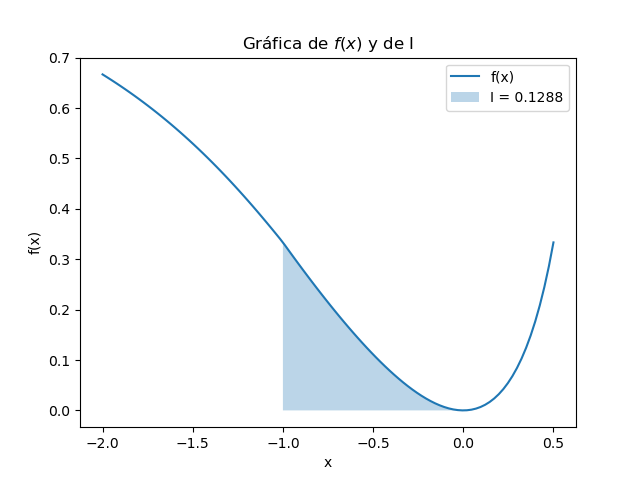
\includegraphics[scale=.6]{EvAU_B2.png}
        \label{fig:enter-label2}
    \end{figure}  
\end{enumerate}

\noindent\rule{\textwidth}{0.5pt}
\newpage
\begin{mybox}
    \paragraph{B.3-} Dada la recta $r\equiv \dfrac{x-1}{2}=\dfrac{y}{1}=\dfrac{z+1}{-2}$, el plano $ \pi : x-z=2$ y el punto $ A(1,1,1)$, se pide:
    \begin{enumerate}
        \item[(a)] Estudiar la posición relativa de $r$ y $\pi$ y calcular su intersección, si existe. 
        \item[(b)] Calcular la proyección ortogonal del punto $A$ sobre el plano $\pi$. 
        \item[(c)] Calcular el punto simétrico del punto $A$ con respecto a la recta $r$. 
    \end{enumerate}
\end{mybox}
\paragraph{Solución:}
\begin{enumerate}
    \item[(a)] Si la intersección entre el plano y la recta da un punto, la posición relativa entre ellos será secantes; si la intersección es la misma recta $r$, entonces $r$ estará contenida en $\pi$; y si la intersección es nula, entonces la recta y el plano son paralelos. Calculamos la intersección: en primer lugar, la recta $r$ en ecuaciones paramétricas es:
    \begin{equation*}
        \begin{split}
        r\equiv \begin{cases}
            x=1+2\lambda& \\
            y=\lambda &,\  \lambda \in \mathbb{R}\\
            z=-1-2\lambda 
            \end{cases}\implies r\cap \pi: x-z&=(1+2\lambda )-(-1-2\lambda )=2\iff \lambda =0 \\
            &\implies \boxed{r\cap \pi =P(1,0,-1)}            
        \end{split}
    \end{equation*}
    Como la intersección es un único punto, la recta y el plano son \textbf{secantes}.

    \item[(b)] Buscamos ahora la proyección ortogonal de $A$ en el plano $\pi$, como aparece representado en el siguiente diagrama:
    
    \begin{minipage}{.4\textwidth}
        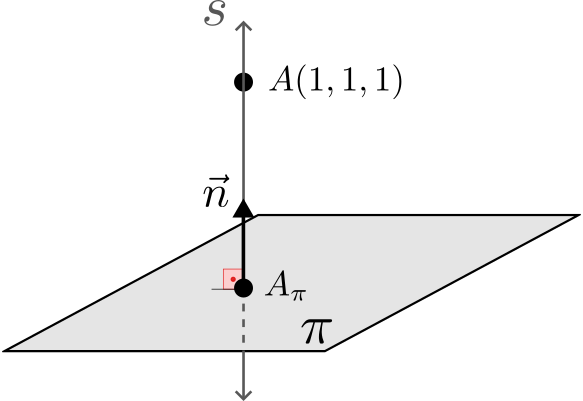
\includegraphics[scale=.35]{b3_b.png}
    \end{minipage}
    \begin{minipage}{.54\textwidth}
        Para encontrar el punto $A_\pi$, trazaremos una recta perpendicular al plano $\pi$ que pase por el punto $A$. Esta recta, $s$, tendrá como vector director $\Vec{u}_s$ el vector normal del plano $\pi$, $\vec{n}=(1,0,-1)$. Por tanto, la recta $s$ tendrá como ecuaciones paramétricas:
        \begin{equation*}
            \begin{split}
               s\equiv  \begin{cases}
                    x=1+\lambda \\
                    y=1\\
                    z=1-\lambda 
                \end{cases}
            \end{split}
        \end{equation*}
    \end{minipage}
    La intersección entre el plano y la recta $s$ es:
    \begin{equation*}
        \begin{split}
            s\cap \pi : x-z=(1+\lambda )-(1-\lambda )=2 \implies \lambda =1 \implies \boxed{A_\pi (2,1,0)}
        \end{split}
    \end{equation*}

    \item[(c)] Buscamos ahora el punto simétrico de $A$, $A'$, con respecto a la recta $r$, como se ve en el dibujo.
    
    \begin{minipage}{.4\textwidth}
        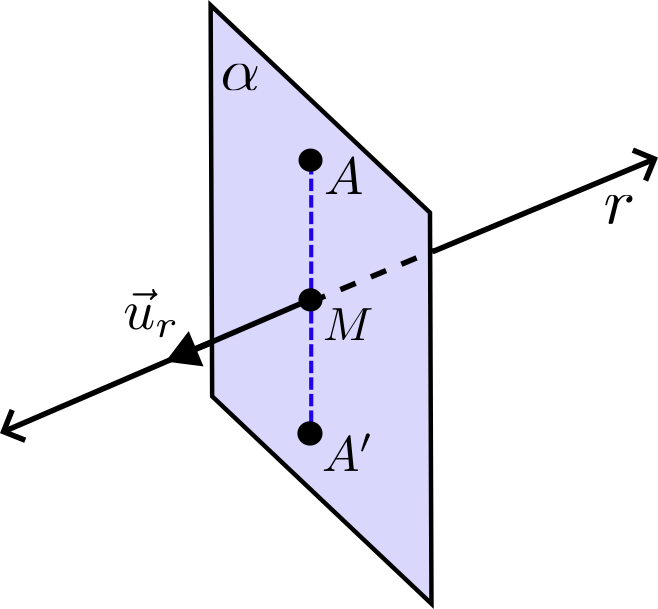
\includegraphics[scale=0.3]{b3_c.png}
    \end{minipage}
    \begin{minipage}{.54\textwidth}
        Para encontrar el punto simétrico $A'$, trazaremos un plano auxiliar $\alpha $ perpendicular a la recta $r$, que tendrá por tanto vector perpendicular $\vec{n}=\vec{u}_r=(2,1,-2)$; y que pase por el punto $A$. La intersección de la recta $r$ con el plano auxiliar nos dará el punto medio entre $A$ y $A'$, $M$. Una vez encontrado el punto $M$, podemos obtener las coordenadas de $A'$ sabiendo que es su punto medio con $A$. En primer lugar, la ecuación del plano auxiliar es:
        \begin{equation*}
            \begin{split}
                \alpha : n_1 x+ n_2 y+n_3 z =2x+y-2z=d
            \end{split}
        \end{equation*}
    \end{minipage}
    
    Sabiendo que el punto $A$ pertenece a $\alpha $, sustituimos las coordenadas de $A$ para encontrar $d$. 
    $$
    2(1)+(1)-2(1)=d=1 \implies \alpha :2x+y-2z=1
    $$
    El punto $M$ es la intersección entre $\alpha $ y $r$: 
    \begin{equation*}
        \begin{split}
            \alpha \cap r: 2x+y-2z=2(1+2\lambda )+ \lambda -2(-1-2\lambda ) &\iff \lambda =-1/3\\
            &\implies M(1/3,-1/3,-1/3)
        \end{split}
    \end{equation*}
    Por último, $M$ es el punto medio de $A$ y $A'$: 
    \begin{equation*}
        \begin{split}
            M=\frac{A+A'}{2} \implies \begin{cases}
                \dfrac{a_1+a_1'}{2}=\dfrac{1+a_1'}{2}=\dfrac{1}{3}&\implies a_1'=-\dfrac{1}{3}\\\\
                \dfrac{a_2+a_2'}{2}=\dfrac{1+a_2'}{2}=-\dfrac{1}{3}&\implies a_2'=-\dfrac{5}{3}\\\\
                \dfrac{a_3+a_3'}{2}=\dfrac{1+a_3'}{2}=-\dfrac{1}{3}&\implies a_3'=-\dfrac{5}{3}
            \end{cases}\\
            \boxed{A'(-1/3,-5/3,-5/3)}
        \end{split}
    \end{equation*}
\end{enumerate}

\noindent\rule{\textwidth}{0.5pt}
\begin{mybox}
    \paragraph{B.4-} La longitud de la sardina del Pacífico (\textit{Sardinops sagax}) se puede considerar que es una variable aleatoria con
distribución normal de media $175$ mm y desviación típica $25.75$ mm.
\begin{enumerate}
    \item[(a)] Una empresa envasadora de esta variedad de sardinas solo admite como sardinas de calidad
aquellas con una longitud superior a $16$ cm. ¿Qué porcentaje de las sardinas capturadas por un buque 
pesquero serán de la calidad que espera la empresa envasadora?  

\item[(b)] Hallar una longitud $t < 175$ mm tal que entre $t$ y $175$ mm estén el 18 $\%$ de las sardinas capturadas. 
\item[(c)]  En altamar se procesan las sardinas en lotes de $10$. Posteriormente se devuelven al mar las
sardinas de cada lote que son menores de $15$ cm por considerarlas pequeñas. ¿Cuál es la probabilidad de
que en un lote haya al menos una sardina devuelta por pequeña?  
\end{enumerate}
\end{mybox}
\paragraph{Solución:}
\begin{enumerate}
    \item[(a)] La variable aleatoria que vamos a estudiar es la 'longitud de las sardinas': \\$X\sim N(\mu =175 \text{ mm}, \sigma =25.75 \text{ mm})$. Estamos interesados en saber el porcentaje de sardinas de calidad admitida, que son aquellas cuya longitud $X>160$ mm. Por tanto, deberemos calcular la probabilidad de que $X>160$, $P(X>160).$ Para ello, primero tipificaremos la distribución normal de $X$.
    \begin{align*}
        X&\longrightarrow Z\sim N(\mu =0 , \sigma =1) & Z\equiv \frac{X-\mu }{\sigma }\\
        P(X>160) &\longrightarrow P\left (Z>\frac{160-\mu }{\sigma }\right )=P(Z>-0.58)&
    \end{align*}
    $$
    P(Z>-0.58)=P(Z<0.58)=0.7190 \quad \text{\footnotesize (mirado en la tabla)}
    $$
    El porcentaje de sardinas de calidad es $\boxed{71.9 \%}$ .

    \item[(b)] Buscamos una longitud $t<175$ mm que cumpla que $P(t<X<175=\mu )=0.18$. Pasando a variable tipificada, esto queda:
    $$
    P\left ( \frac{t-\mu }{\sigma }<Z<0 \right )=\underbrace{P(Z<0)}_{0.5}-P\left (Z<\frac{t-\mu }{\sigma } \right )=0.18 \implies P\left (Z<\frac{t-\mu }{\sigma } \right )=0.32
    $$
    Como $(t-\mu) /\sigma $ es negativo, tenemos que convertirlo a un valor positivo. 
    \begin{equation*}
        \begin{split}
            P\left (Z<\frac{t-\mu }{\sigma } \right ) = 1- P\left (Z<\frac{\mu -t }{\sigma } \right )&\implies P\left (Z<\frac{\mu -t }{\sigma } \right )=0.68\\
            &\implies Z=0.47 \quad \text{\footnotesize (valor de probabilidad más cercano es $0.6808$)} \\&\implies \boxed{t\approx 162 \text{ mm}}
        \end{split}
    \end{equation*}

    \item[(c)] La 'sardina procesada' ($X$) es una variable que toma dos valores: o bien es devuelta por pequeña ($X=1$) o bien no es devuelta ($X=0$). Por tanto, $X\sim \text{Ber}(p=P(X<150))$. Esta probabilidad $p$ se calcula de la misma forma que hemos venido haciendo.
    $$
    p=P(X<150)=P(Z<-0.97)=1-P(Z<0.97)=0.166
    $$
    La variable $Y$ 'sardinas pequeñas en lotes de $n=10$' sigue una distribución binormal:\\ $Y\sim \text{Bin}(n=10,p=0.166)$. La probabilidad de que al menos una sardina haya sido devuelta es:
    $$
    P(Y\ge 1)=1-P(Y=0)=1-\binom{10}{0}p^0 (1-p)^{10} = 1-(1-0.166)^{10}=\boxed{0.8372}
    $$
\end{enumerate} 

\noindent\rule{\textwidth}{0.5pt}

\end{document}
